\subsection{SGX Software Attestation}
\label{sec:sgx_attestation}

The software attestation scheme implemented by SGX follows the principles
outlined in \S~\ref{sec:generic_software_attestation}. An SGX-enabled processor
computes a measurement of the code and data that is loaded in each enclave,
which is similar to the measurement computed by the TPM~(\S~\ref{sec:tpm}). The
software inside an enclave can start a process that results in an SGX
attestation signature, which includes the enclave's measurement and an enclave
message.

However, the software attestation scheme in SGX's design, summarized in
Figure~\ref{fig:sgx_attestation_overview} is unnecessarily complicated by the
decision to deeply couple software attestation with
\textbf{an enclave licensing mechanism that allows Intel to force itself as an
intermediary in the distribution of all enclave software}.

\begin{figure}[hbt]
  \centering
  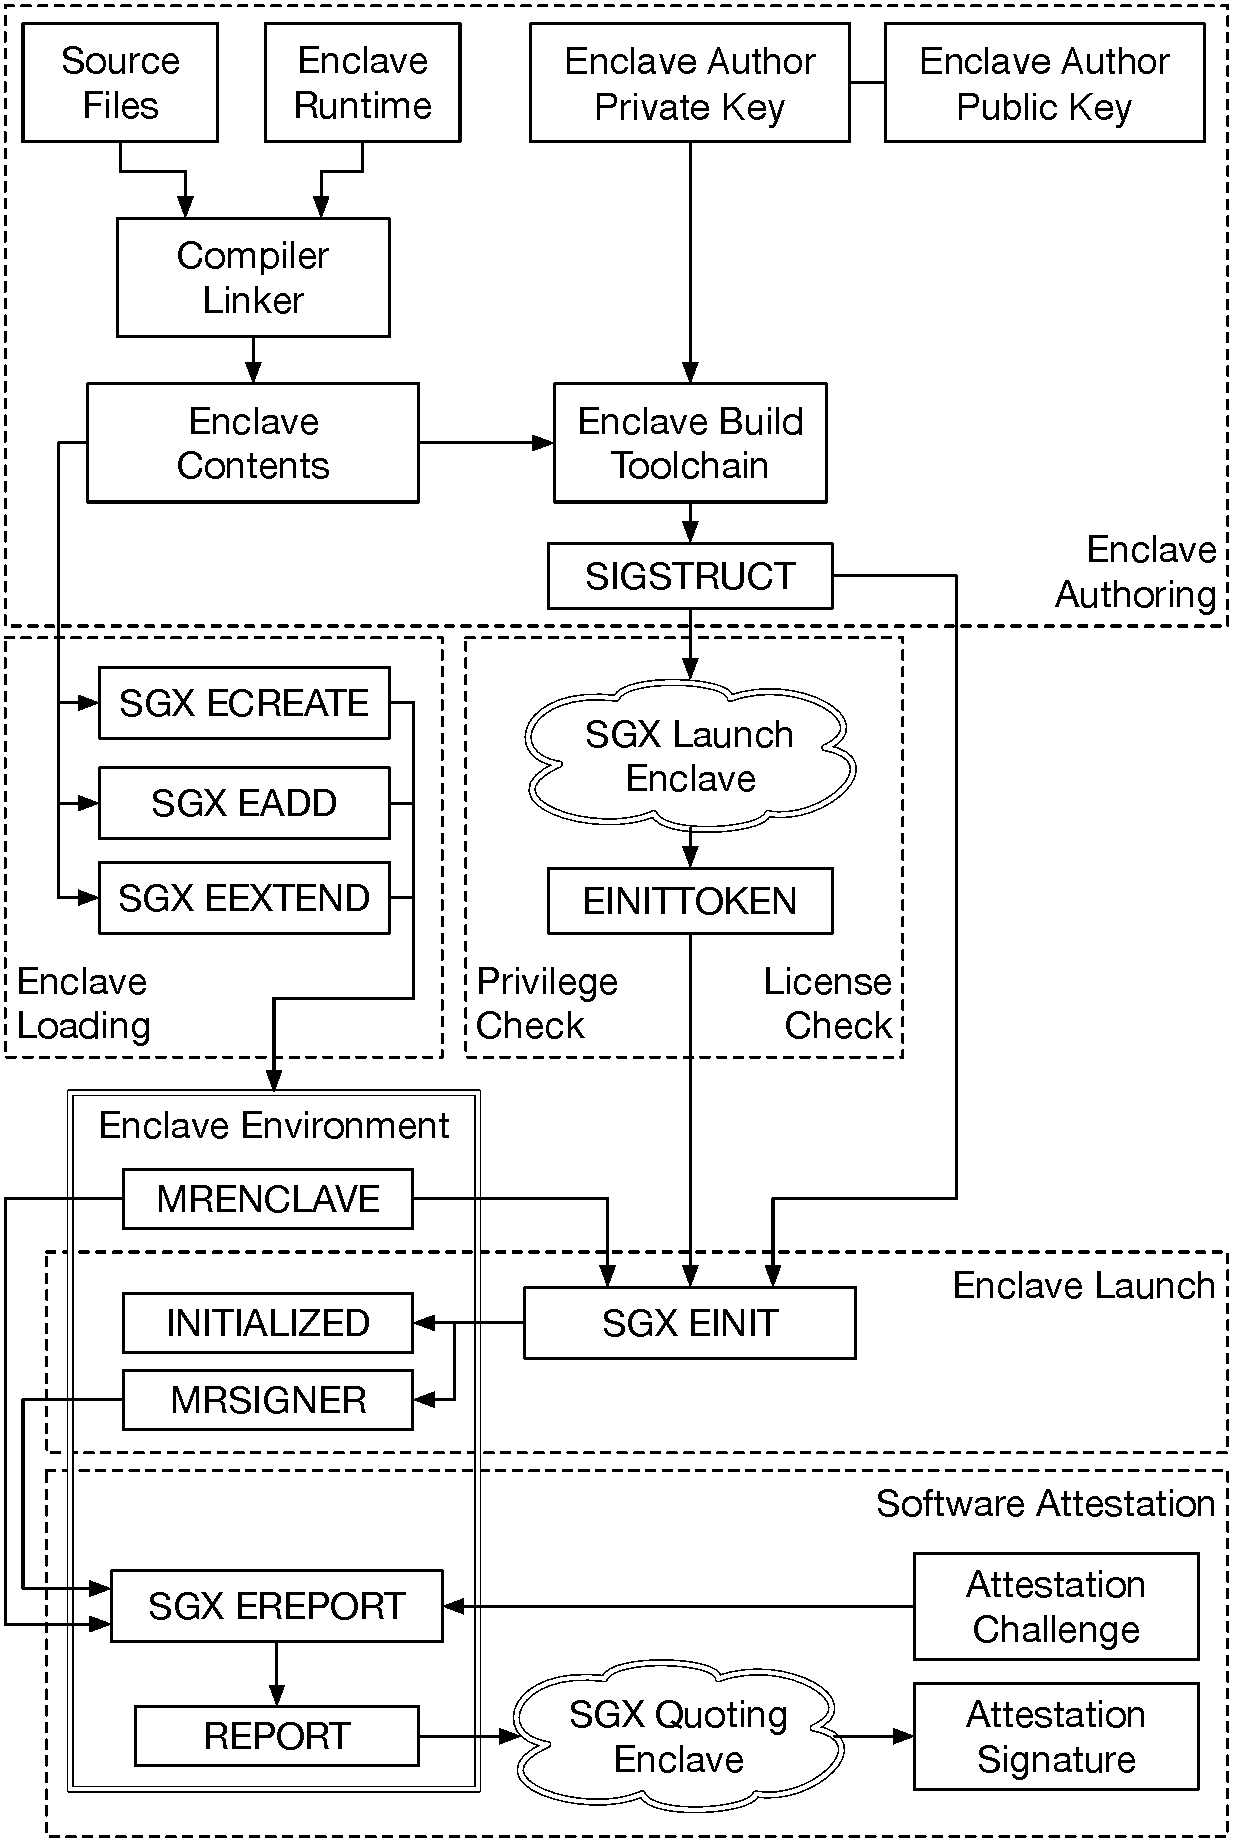
\includegraphics[width=85mm]{figures/sgx_attestation_overview.pdf}
  \caption{
    Setting up an SGX enclave and undergoing the software attestation process
    involves the SGX instructions \texttt{EINIT} and \texttt{EREPORT}, and two
    special enclaves authored by Intel, the SGX Launch Enclave and the SGX
    Quoting Enclave.
  }
  \label{fig:sgx_attestation_overview}
\end{figure}

Initializing an enclave via \textit{EINIT}~(\S~\ref{sec:sgx_einit_overview})
generally requires an \texttt{EINIT} Token structure~(EINITTOKEN), which can
only be issued by the SGX Launch enclave, as described in
\S~\ref{sec:sgx_launch_enclave}. The SDM does not specify the role of the
Launch Enclave, but one of the SGX patents~\cite{intel2013patent1} discloses in
no uncertain terms that the Launch Enclave is intended to check that the
enclave author has a business relationship with Intel.

After an enclave gets cleared by the SGX Launch Enclave and is initialized via
\texttt{EINIT}, it can authenticate itself to a remote party by participating
in a software attestation process. This is a two-step process. First, the
enclave uses the \texttt{EREPORT} instruction to create a REPORT structure,
described in \S~\ref{sec:sgx_ereport}. This structure only proves the enclave's
identity to the SGX Quoting Enclave, described in
\S~\ref{sec:sgx_quoting_enclave}, which is a special enclave authored by Intel
that can access to the CPU's attestation key. Therefore, the REPORT structure
created by \texttt{EREPORT} is given to the SGX Quoting Enclave, which produces
an attestation signature that can be verified by a remote party.

The EINITTOKEN and REPORT structures are passed between enclaves by untrusted
system software, so they require integrity guarantees. The structures'
integrity is assured by a MAC scheme~(\S~\ref{sec:integrity_crypto}) that uses
symmetric keys supplied by the SGX key derivation feature described in
\S~\ref{sec:sgx_egetkey}.








\subsubsection{License Verification}
\label{sec:sgx_launch_enclave}

% ATTRIBUTES: SDM S 38.7.1
% EINIT: SDM S 41.3
% EINITTOKENKEY is bit 5, INTEL_ONLY_MASK is 0x20

% EINIT Token Structure (EINITTOKEN): SDM S 38.14

\begin{figure}[hbt]
  \centering
  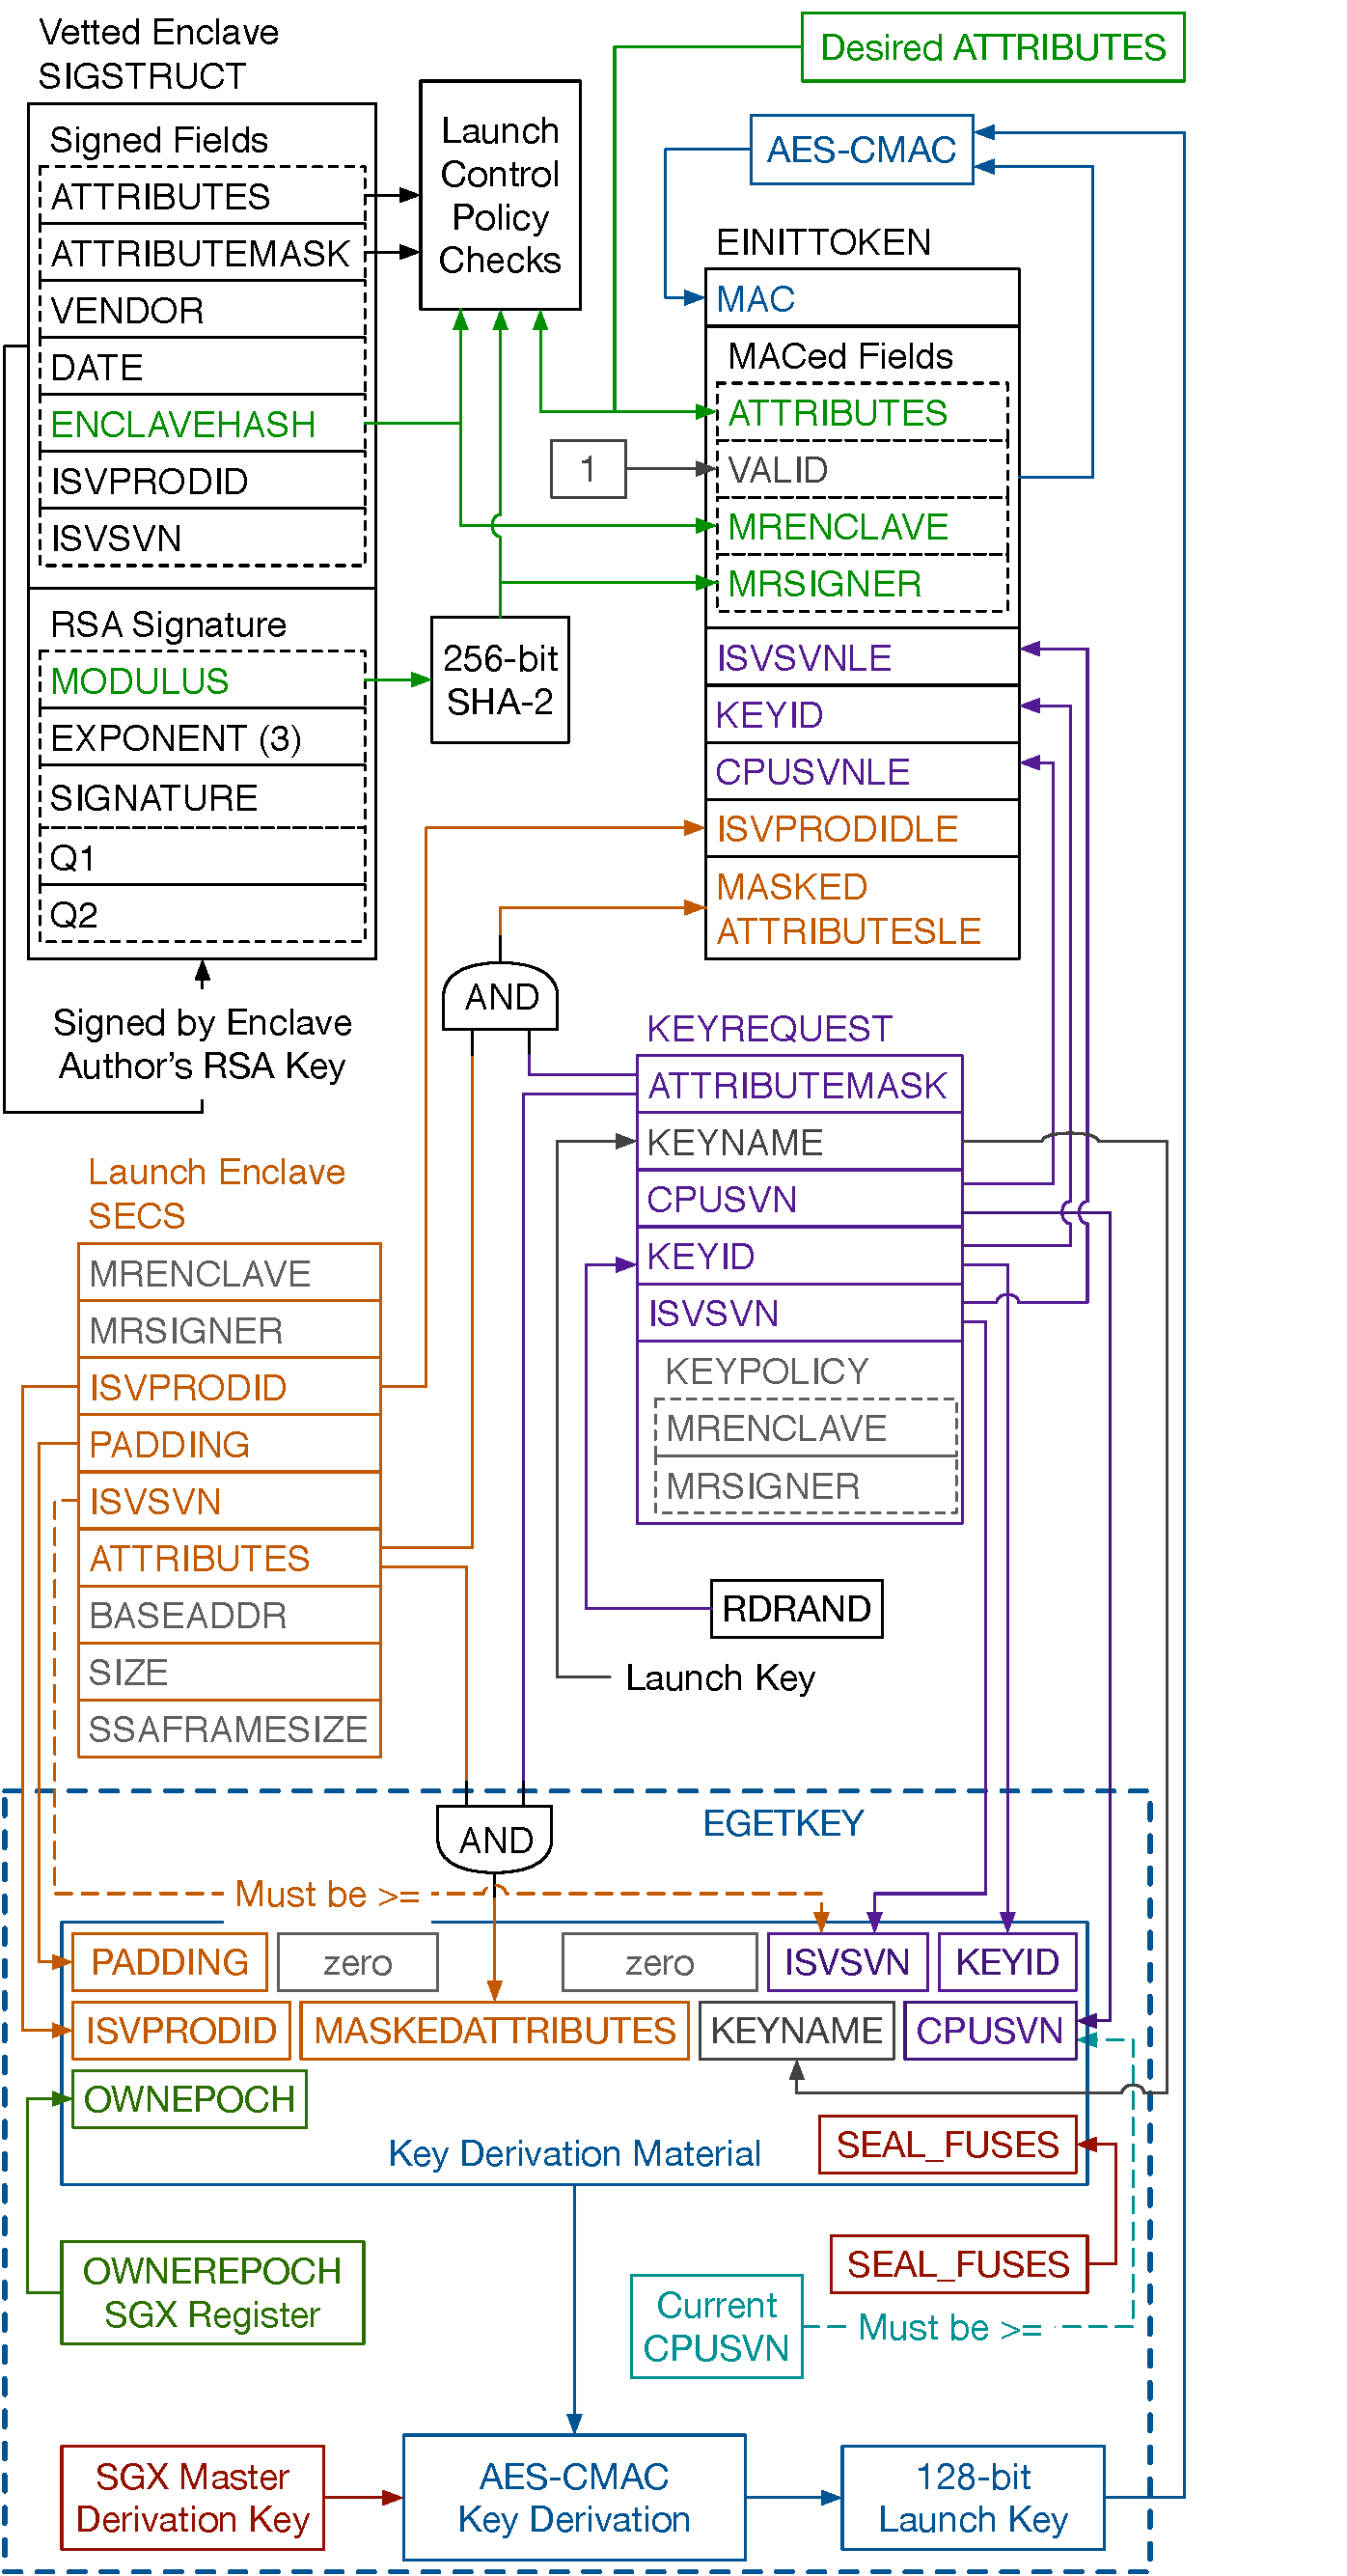
\includegraphics[width=87mm]{figures/sgx_einittoken.pdf}
  \caption{
    The SGX Launch Enclave computes the EINITTOKEN.
  }
  \label{fig:sgx_einittoken}
\end{figure}

The SDM states that the MAC that protects EINITTOKEN's authenticity is computed
using a block cipher-based MAC~(CMAC,~\cite{fips2005cmac}), but stops short of
specifying the underlying cipher. One of the SGX papers~\cite{anati2013sgx}
states that SGX implementation uses a CMAC based on 128-bit AES.



\subsubsection{Inter-Enclave Attestation}
\label{sec:sgx_ereport}

The enclave asks the CPU to produce an \textit{enclave report}, which contains
the attestation challenge, the enclave's measurement value, an
enclave-generated 256-byte message, and an HMAC
 with a symmetric key shared between the CPU and a special
\textit{signing enclave} produced by Intel. The untrusted system software
executes the signing enclave, which verifies the report and produces an
\textit{attestation signature} that covers the challenge and the enclave's
measurement.


\subsubsection{Enclave Initialization}
\label{sec:sgx_einit}

% MRSIGNER: SDM S 39.4.1.2

\texttt{EINIT}~(\S~\ref{sec:sgx_einit_overview}) requires the virtual address
of the SIGSTRUCT associated with the enclave to be initialized. The instruction
checks the validity of SIGSTRUCT's contents, and refuses to proceed if it
detects inconsistencies. For example, \texttt{EINIT} verifies the RSA
signature and returns an error code if the signature is invalid.

\texttt{EINIT} computes a 256-bit SHA-2 hash of the RSA exponent in the
enclave's SIGSTRUCT, and writes it into the MRSIGNER field in the enclave's
SECS. For this reason, the RSA exponent's hash is referred to as MRSIGNER
throughout the SGX documentation. This value is the cryptographic identity of
the enclave's author.

The \texttt{EINIT} instruction also copies the ISVPRODID and ISVSVN fields from
SIGSTRUCT into the enclave's SECS. In the scope of SGX's key generation
feature, which will be discussed in \S~\ref{sec:sgx_egetkey}, all the enclaves
that have the same MRSIGNER and ISVPRODID represent different versions of the
same software, and are ordered according to the value of the ISVSVN field.
Higher ISVSVN values identify newer enclave versions that potentially fix
security vulnerabilities found in the older versions.


\subsubsection{The Quoting Enclave}
\label{sec:sgx_quoting_enclave}

